\documentclass[11pt]{article}
\usepackage{euscript}

\usepackage{amsmath}
\usepackage{amsthm}
\usepackage{amssymb}
\usepackage{epsfig}
\usepackage{xspace}
\usepackage{color}
\usepackage{url}

%%%%%%%%%%%%%%%%%%%%%%%%%%%%%%%%%
\setlength{\textheight}{9in}
\setlength{\topmargin}{-0.600in}
\setlength{\headheight}{0.2in}
\setlength{\headsep}{0.250in}
\setlength{\footskip}{0.5in}
\flushbottom
\setlength{\textwidth}{6.5in}
\setlength{\oddsidemargin}{0in}
\setlength{\evensidemargin}{0in}
\setlength{\columnsep}{2pc}
\setlength{\parindent}{1em}
%%%%%%%%%%%%%%%%%%%%%%%%%%%%%%%%%


\newcommand{\eps}{\varepsilon}

\renewcommand{\c}[1]{\ensuremath{\EuScript{#1}}}
\renewcommand{\b}[1]{\ensuremath{\mathbb{#1}}}
\newcommand{\s}[1]{\textsf{#1}}

\newcommand{\E}{\textbf{\textsf{E}}}
\renewcommand{\Pr}{\textbf{\textsf{Pr}}}

\title{HW04: Utility and Markov Decision Processes
\footnote{\s{CS 5300 AI; \;\; Spring 2012 \hfill
Instructor: Jur van den Berg, University of Utah}
}
}
\author{Alex Clemmer, u0458675}

\begin{document}
\maketitle





%%%%%%%%%%%%%%%%%%%%%%%%%%%%%%%%%%%%%%%%%%%%%%%%%%%%
%%%%%%%%%%%%%%%%%%%%%%%%%%%%%%%%%%%%%%%%%%%%%%%%%%%%
%%%%%%%%%%%%%%%%%%%%%%%%%%%%%%%%%%%%%%%%%%%%%%%%%%%%
\section{Utility and Expectation}

\begin{enumerate}
    \item Coin toss lottery. Let $P$ be the random variable representing the amount of money won from the coin toss. Let $\Pr(F_H)$ stand for the probability of flipping heads, and $\Pr(G_H)$ stand for the probability of guessing heads. 
    
    \begin{enumerate}
      \item If we assume that guessing heads or tails is equally likely, the probability of correctly guessing an already-flipped coin is simply 0.5; that is, $\Pr(G_H \cap F_H) + \Pr(G_T \cap F_T) = 0.25 + 0.25$.
      
      Thus, the expectation of payoff $P$ is $\E[P] = \$3 \cdot \Pr(G_H \cap F_H) + \$3 \cdot \Pr(G_T \cap F_T) + \$0 \cdot \Pr(G_H \cap F_T) + \$0 \cdot \Pr(G_T \cap F_T) = \mathbf{\$1.5}$
      
      
      \item The probabilities don't change, but the values do: $\E[P] = \$3 \cdot \Pr(G_H \cap F_H) + \$8 \cdot \Pr(G_T \cap F_T) + \$0 \cdot \Pr(G_H \cap F_T) + \$0 \cdot \Pr(G_T \cap F_T) = \$0 \cdot 0.25 + \$0 \cdot 0.25 + \$3 \cdot 0.25 + \$8 \cdot 0.25 = \mathbf{\$2.75}$
      
      \item I'll assume the payouts are the same as in (b), though this is not explicitly stated. Then: $\E[P] = \$0 \cdot \Pr(G_T \cap F_H) + \$8 \cdot \Pr(G_T \cap F_T) + \$3 \cdot \Pr(G_H \cap F_H) + \$0 \cdot \Pr(G_T \cap F_H) = \$0 \cdot 0.5 + \$8 \cdot 0.5 + \$3 \cdot 0.0 + \$0 \cdot 0.0 = $ \$ $\mathbf{4}$.
    \end{enumerate}
    
    \item The problem is a bit unclear, so I'll just assume that Tom pays Bob ahead of time, and then if Tom wins, Bob will pay back \textit{double} what Tom initially paid --- that is, Tom pays 100\% of the wager ahead of time and then, if he is right, he recieves 200\% of what he wagered, for a net total of 100\% of the wager (and \textit{not} 100\% of what he wagered plus 200\% of that wager).
    
    Further, I assume both that $\Pr(Roll_1) = \Pr(Roll_3)$, and that $\Pr(Roll_2) = \Pr(Roll_4)$ --- that is to say, I assume that the probability of a number being even is equally distributed among even numbers (and the same for odd). Also note that $\Pr(A \cap B) = \Pr(A|B)P(B)$.
    
    Then the expectations are as follows:
    
    $\E[Guess_1] = 1 \cdot \Pr(Roll_1) \cdot \Pr(Guess_1 | Roll_1) + -2 \cdot \Pr(Roll_2) \cdot \Pr(Guess_1 | Roll_2) + -3 \cdot \Pr(Roll_3) \cdot \Pr(Guess_1 | Roll_3) + -4 \cdot \Pr(Roll_4) \cdot \Pr(Guess_1 | Roll_4) = 1(1/6)(1/4) + -2(1/3)(1/4) + -3(1/6)(1/4) + -4(1/3)(1/4) = \textbf{-7/12 dollars}$
    
    $\E[Guess_2] = -1 \cdot \Pr(Roll_1) \cdot \Pr(Guess_1 | Roll_1) + 2 \cdot \Pr(Roll_2) \cdot \Pr(Guess_1 | Roll_2) + -3 \cdot \Pr(Roll_3) \cdot \Pr(Guess_1 | Roll_3) + -4 \cdot \Pr(Roll_4) \cdot \Pr(Guess_1 | Roll_4) = -1(1/6)(1/4) + 2(1/3)(1/4) + -3(1/6)(1/4) + -4(1/3)(1/4) = \textbf{-1/3 dollars}$
    
    $\E[Guess_3] = -1 \cdot \Pr(Roll_1) \cdot \Pr(Guess_1 | Roll_1) + -2 \cdot \Pr(Roll_2) \cdot \Pr(Guess_1 | Roll_2) + 3 \cdot \Pr(Roll_3) \cdot \Pr(Guess_1 | Roll_3) + -4 \cdot \Pr(Roll_4) \cdot \Pr(Guess_1 | Roll_4) = -1(1/6)(1/4) + -2(1/3)(1/4) + 3(1/6)(1/4) + -4(1/3)(1/4) = \textbf{-5/12 dollars}$
    
    $\E[Guess_4] = -1 \cdot \Pr(Roll_1) \cdot \Pr(Guess_1 | Roll_1) + -2 \cdot \Pr(Roll_2) \cdot \Pr(Guess_1 | Roll_2) + -3 \cdot \Pr(Roll_3) \cdot \Pr(Guess_1 | Roll_3) + 4 \cdot \Pr(Roll_4) \cdot \Pr(Guess_1 | Roll_4) = -1(1/6)(1/4) + -2(1/3)(1/4) + -3(1/6)(1/4) + 4(1/3)(1/4) = \textbf{0 dollars}$
    
    \item N/A

    \item Given all this, the actual calculation involves a fairly annoying application of the products of probabilities. Note that because the probability that the guess is some number and the probability of the roll is some number are not independent, we thus have to total all the cases somewhat tediously; consider, for example, the probability that Bob gains \$1 is totaled as $\Pr(Roll_3) \cdot \Pr(Guess_1 | Roll_3) + \Pr(Roll_{even}) \cdot \Pr(Guess_1 | Roll_{even})$, since when we roll 1 and guess 1, Bob pays Tom \$1. Also, remember, given the assumptions above, $\Pr(Roll_1) = \Pr(Roll_3) = 1/6$ and $\Pr(Roll_2) = \Pr(Roll_4) = 1/3$. I also assume that all guesses are equiprobable.
    
    The explicit equation is thus this monstrosity: $\E[P] = -\$1 \cdot \Pr(Roll_1) \cdot \Pr(Guess_1 | Roll_1) + -\$2 \cdot \Pr(Roll_2) \cdot \Pr(Guess_2 | Roll_2) + -\$3 \cdot \Pr(Roll_3) \cdot \Pr(Guess_3 | Roll_3) + -\$4 \cdot \Pr(Roll_4) \cdot \Pr(Guess_4 | Roll_4) + \$1 \cdot \Pr(Roll_{3}) \cdot \Pr(Guess_1 | Roll_{3}) + \$1 \cdot \Pr(Roll_{even}) \cdot \Pr(Guess_1 | Roll_{even}) + \$2 \cdot \Pr(Roll_{odd}) \cdot \Pr(Guess_2 | Roll_{odd}) + \$2 \cdot \Pr(Roll_{4}) \cdot \Pr(Guess_2 | Roll_{4}) + \$3 \cdot \Pr(Roll_{1}) \cdot \Pr(Guess_3 | Roll_{1}) + \$3 \cdot \Pr(Roll_{even}) \cdot \Pr(Guess_3 | Roll_{even}) + \$4 \cdot \Pr(\neg Roll_{odd}) \cdot \Pr(Guess_4 | Roll_{odd}) + \$4 \cdot \Pr(\neg Roll_{2}) \cdot \Pr(Guess_4 | Roll_{2})$
    
    \textbf{This all translates to this awful expected value calculation:} $\E[P] = (1/6)(1/4)(-\$1) + (1/6)(1/4)(-\$3) + (1/3)(1/4)(-\$2) + (1/3)(1/4)(-\$4) + (1/6)(1/4)\$1 + 2(1/3)(1/4)\$1 + 2(1/6)(1/4)\$2 + (1/3)(1/4)\$2 + (1/6)(1/4)\$3 + 2(1/3)(1/4)\$3 + 2(1/6)(1/4)\$4 + (1/3)(1/4)\$4 = \mathbf{\$7/6} \approx $\$ $ \mathbf{1.16667}$

\end{enumerate}

\section{AIMA Problem 17.8}

\textbf{NOTE:} I am assuming That $r$ is not an exit node, since in the figure, it does not have a box around it.

\begin{enumerate}
\item Case: $r = 300$. The agent in this case really wants to move to the $r$ cell because the reward is so incredibly high. Although the actor will not explicitly avoid going to the exit simply because it is an exit, in this case, the center cell is next to \textit{two} nodes that lead directly to $r$, and so typically its utility will be higher than the exit node even though its reward is positive. Thus, even the node directly beneath it will not point directly at it. (For reference, I actually did run the algorithm to make sure.)

\begin{center}
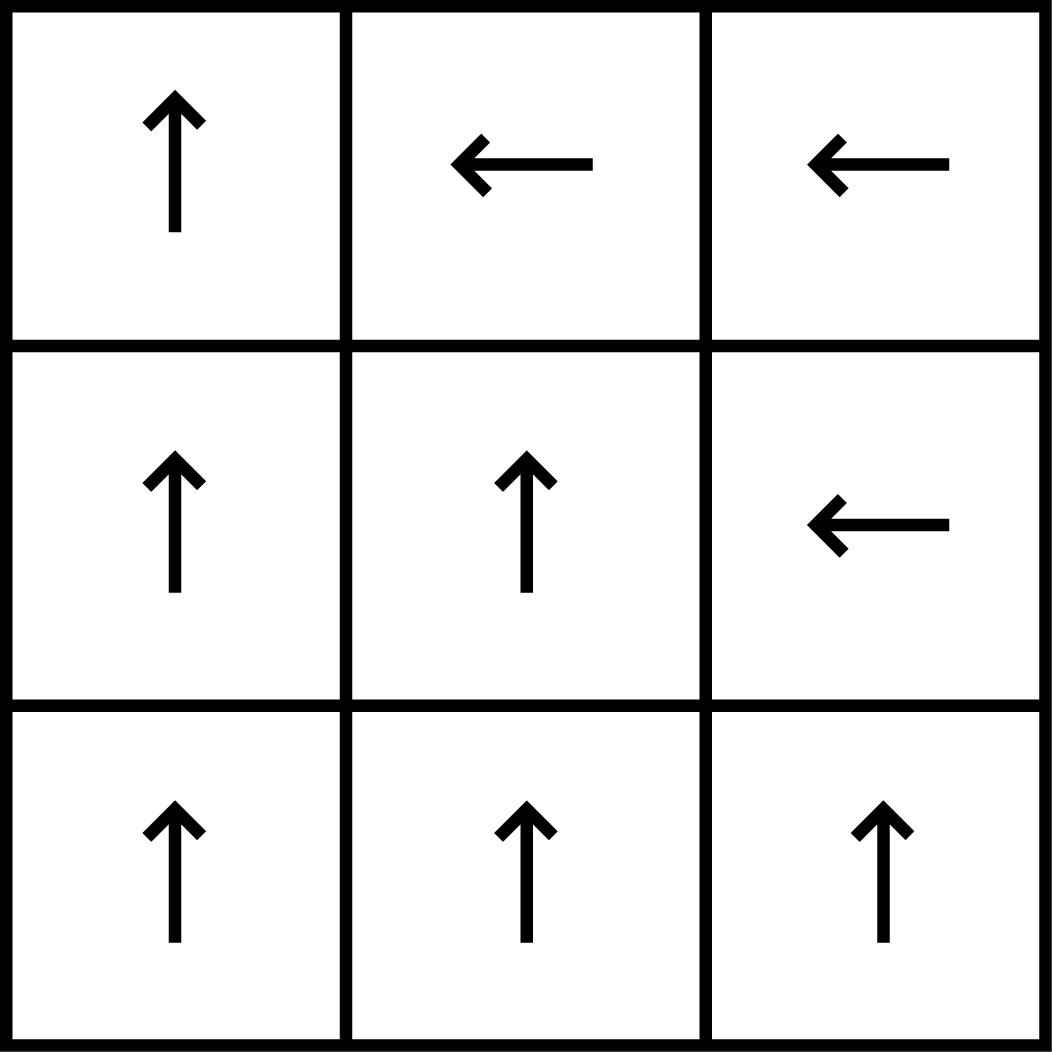
\includegraphics[scale=0.25]{300.png}
\end{center}

\item Case: $r = -3$. Unlike the first problem, the agent here wants to exit as quickly as possible, since the $r$ cell provides no incentive to stick around. Again the center cell will be right next to paths that lead directly to the exit (which is the highest-value cell), and therefore the cell beneath the $r$ cell will point to it, because ultimately the incentive to point away from the $r$ cell is not great enough to cause it to point away from the center cell. (I also ran this to make sure.)

\begin{center}
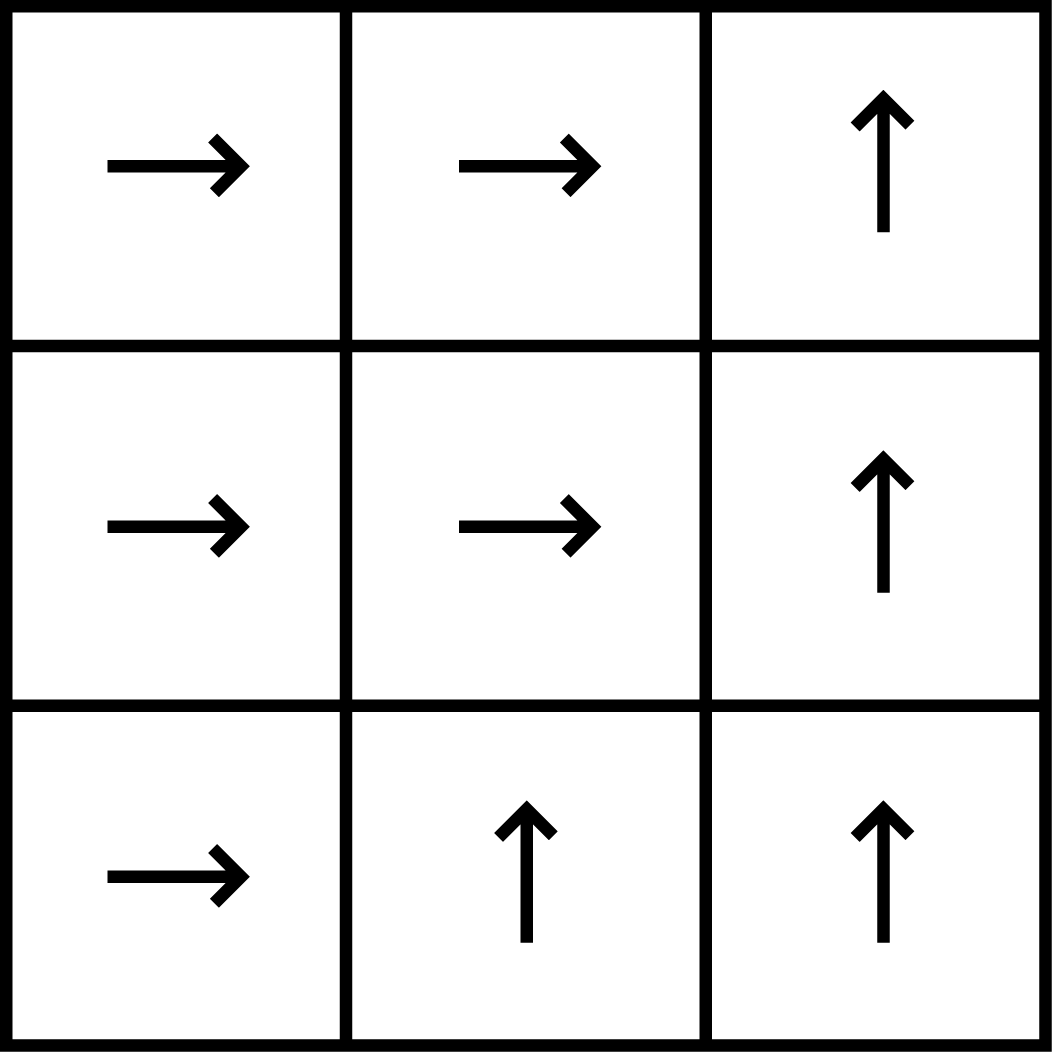
\includegraphics[scale=0.25]{n3.png}
\end{center}

\item Case: $r = 0$. Rhe cell directly beneath the $r$ cell will actually point towards the $r$ cell. It seems like the center cell, which is connected to \textit{two} cells that point directly at the exit cell, would take precedence, but it does not provide the path of least resistance, and when you actually run it, the path generated goes through the $r$ node. The rest is as one would expect it.

\begin{center}
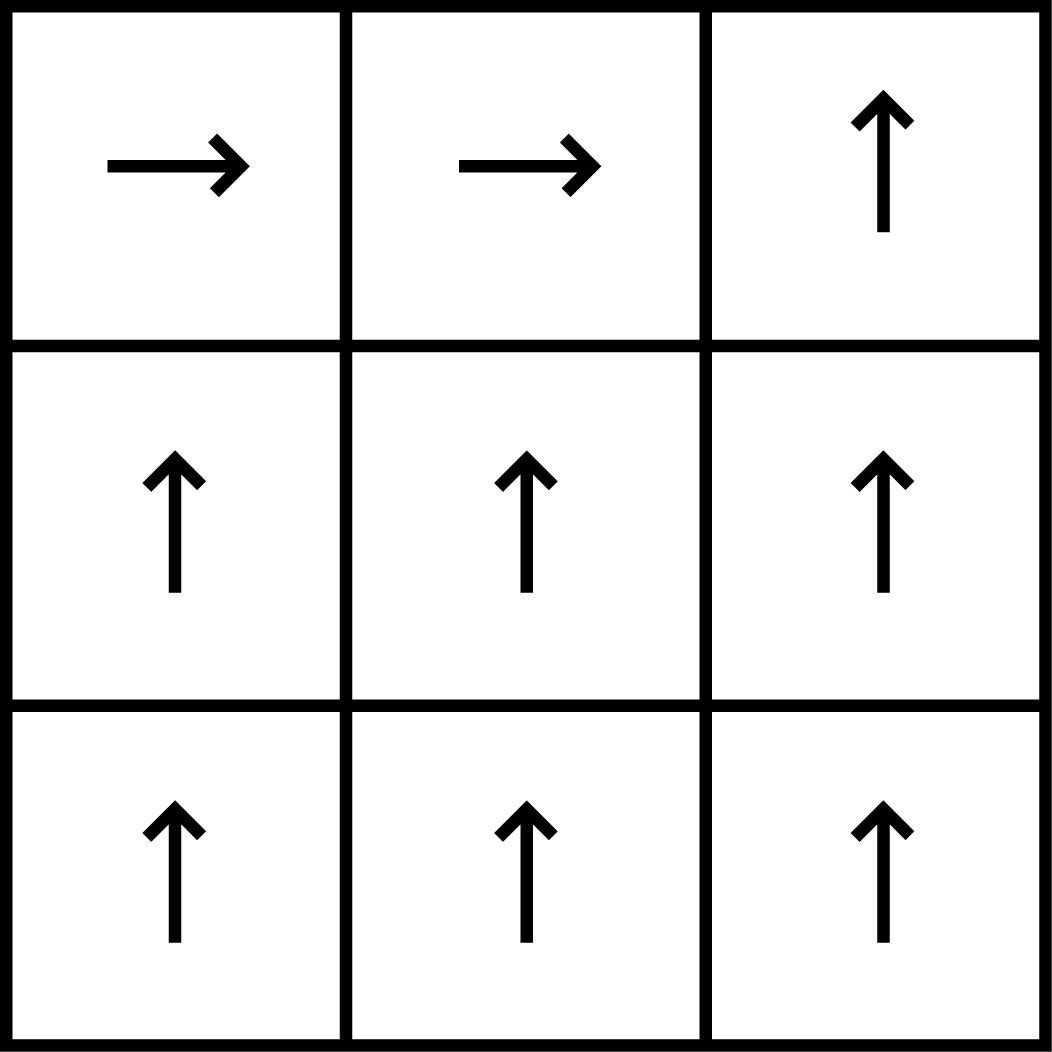
\includegraphics[scale=0.25]{0.png}
\end{center}

\item Case: $r = 3$. Although an agent could theoretically stick around and try to stay inside the $r$ cell, forever obtaining increase in score, it will not. If it has the oppotunity, it will go through the $r$ cell, but it will then proceed towards the exit, which has the greatest payoff. This is because of the fact that it is an exit cell does not actually factor into the algorithm.

\begin{center}
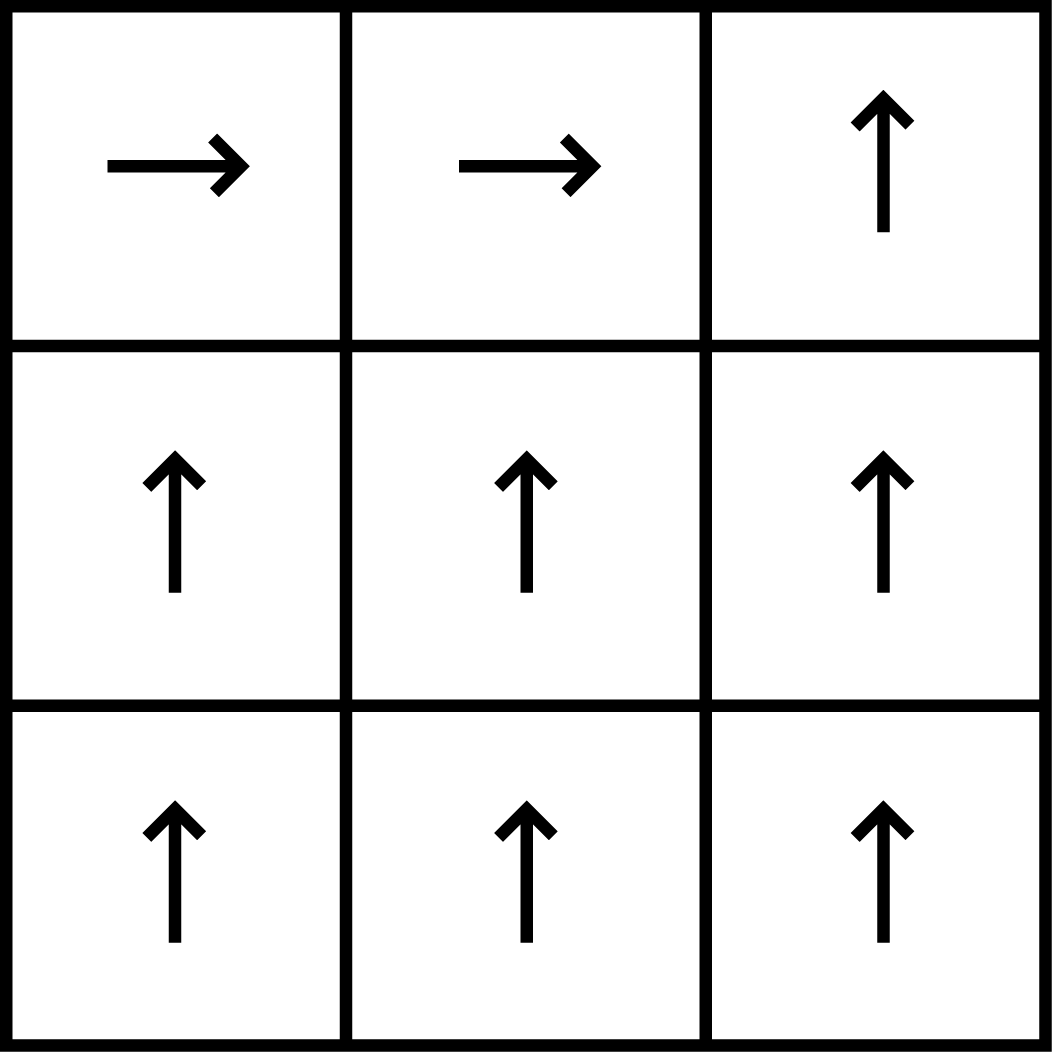
\includegraphics[scale=0.25]{3.png}
\end{center}

\end{enumerate}

\section{Mission to Mars}

\begin{enumerate}
\item There are 4 deterministic policies: (1) the \textit{all-slow} policy, which goes slow no matter what; (2) the \textit{all-fast} policy, which goes fast no matter what; and (3) the \textit{alternating} policy, which starts out going fast in the cool state, and then slows down once it reaches the warm state.

Note that the last policy is somewhat silly: (4) is an alternating policy as well, but instead of going fast in the cool state and slow in the warm state, it goes slow in the cool state and fast in the warm state. This is meaningless because going slow in the cool state transitions back to the cool state 100\% of the time, so we never actually get to the warm state. But I treat this as a distinct policy because there is no other policy that gives the same recommendations over all the possible states.

\item \textit{Much} higher than the warm state.

\item I chose to use the standard \textbf{Bellman Equation}-derived Value Iteration update rule (as noted in the book), rather than the equation in Dustin's notes, which comes from Wikipedia. They are totally equivalent, but for reference, the Bellman-derived rule looks like this: $U_{i+1} \leftarrow R(s) + \gamma \underset{a \in A(s)}{\max} \sum_{s'} P(s' | a, s) U_i(s')$.

  \begin{tabular}{ | c | c | c | c | }
    \hline
    $s$ & $V_0(s)$ & $V_1(s)$ & $V_2(s)$ \\ \hline
    cool & 0 & \textbf{10} & \textbf{19} \\ \hline
    warm & 0 & \textbf{10} & \textbf{17.875} \\ \hline
    off & 0 & 0 & 0 \\
    \hline
  \end{tabular}

\item Technically speaking, without a finite horizon, this will converge as part of an infinite series. We usually ameliorate this concern by picking some $\epsilon$ and stopping the iteration at that point.

\item After 7 iterations or so, the optimal policy begins to recommend \textit{alternation}: if you're in the cool state, you should go fast, and if you're in the warm state, you should go slow.

  \begin{tabular}{ | c | c | }
    \hline
    $s$ & $\pi(s)$ \\ \hline
    cool & fast \\ \hline
    warm & slow \\
    \hline
  \end{tabular}

\item After 7 iterations, I get:

  \begin{tabular}{ | c | c | }
    \hline
    $s$ & $V^*(s)$ \\ \hline
    cool & 43.2834 \\ \hline
    warm & 38.3154 \\ \hline
    off & 0 \\
    \hline
  \end{tabular}

\end{enumerate}






\end{document}
